% !TEX encoding = UTF-8 Unicode
%%%%%%%%%%%%%%%%%%%%%%%%%%%%%%%%%%%%%%%%%
% Beamer Presentation
% LaTeX Template
% Version 1.0 (10/11/12)
%
% This template has been downloaded from:
% http://www.LaTeXTemplates.com
%
% License:
% CC BY-NC-SA 3.0 (http://creativecommons.org/licenses/by-nc-sa/3.0/)
%
%%%%%%%%%%%%%%%%%%%%%%%%%%%%%%%%%%%%%%%%%

%----------------------------------------------------------------------------------------
%	PACKAGES AND THEMES
%----------------------------------------------------------------------------------------

\documentclass{beamer}

\mode<presentation> {

% The Beamer class comes with a number of default slide themes
% which change the colors and layouts of slides. Below this is a list
% of all the themes, uncomment each in turn to see what they look like.

%\usetheme{default}
%\usetheme{AnnArbor}
%\usetheme{Antibes}
%\usetheme{Bergen}
%\usetheme{Berkeley}
%\usetheme{Berlin}
%\usetheme{Boadilla}
%\usetheme{CambridgeUS}
%\usetheme{Copenhagen}
%\usetheme{Darmstadt}
%\usetheme{Dresden}
%\usetheme{Frankfurt}
%\usetheme{Goettingen}
%\usetheme{Hannover}
%\usetheme{Ilmenau}
%\usetheme{JuanLesPins}
%\usetheme{Luebeck}
%\usetheme{Madrid}
%\usetheme{Malmoe}
%\usetheme{Marburg}
%\usetheme{Montpellier}
%\usetheme{PaloAlto}
%\usetheme{Pittsburgh}
%\usetheme{Rochester}
\usetheme{Singapore}
%\usetheme{Szeged}
%\usetheme{Warsaw}

% As well as themes, the Beamer class has a number of color themes
% for any slide theme. Uncomment each of these in turn to see how it
% changes the colors of your current slide theme.

%\usecolortheme{albatross}
%\usecolortheme{beaver}
%\usecolortheme{beetle}
%\usecolortheme{crane}
%\usecolortheme{dolphin}
%\usecolortheme{dove}
%\usecolortheme{fly}
%\usecolortheme{lily}
%\usecolortheme{orchid}
%\usecolortheme{rose}
%\usecolortheme{seagull}
%\usecolortheme{seahorse}
%\usecolortheme{whale}
%\usecolortheme{wolverine}

%\setbeamertemplate{footline} % To remove the footer line in all slides uncomment this line
%\setbeamertemplate{footline}[page number] % To replace the footer line in all slides with a simple slide count uncomment this line

%\setbeamertemplate{navigation symbols}{} % To remove the navigation symbols from the bottom of all slides uncomment this line
}

\usepackage{graphicx} % Allows including images
\usepackage{booktabs} % Allows the use of \toprule, \midrule and \bottomrule in tables
\usepackage{xeCJK}
\setCJKmainfont{SourceHanSerif-Regular}
\usepackage{color}
\usepackage{listings}
\lstset{numbers=left}
\usepackage{fancyvrb}%use Verbatim-the extended verbatim
\usepackage{tikz}


%----------------------------------------------------------------------------------------
%	TITLE PAGE
%----------------------------------------------------------------------------------------

\title[Django]{python} % The short title appears at the bottom of every slide, the full title is only on the title page
\subtitle{Introduce}
\author{} % Your name
\institute[计算机科学与技术学院] % Your institution as it will appear on the bottom of every slide, may be shorthand to save space
{
贵州大学 \\ % Your institution for the title page
\medskip
\textit{hnzhang1@gzu.edu.cn} % Your email address
}
\date{\today} % Date, can be changed to a custom date

\begin{document}

\begin{frame}
\titlepage % Print the title page as the first slide
\end{frame}
\begin{frame}{Overview}
\tableofcontents
\end{frame}
\section{Introduction}
\begin{frame}{}

\includegraphics{python-logo.png}
python是一门比较容易入门、流行、解释型、面向对象、跨平台的的语言。

网上学习资源推荐:\url{https://www.icourse163.org/course/BIT-268001}
\end{frame}
\begin{frame}{install}
\begin{enumerate}
\item
版本:python 3.x
\item
系统平台:根据自己的实际情况选择
\begin{itemize}
\item
\textcolor{red}{Linux}
\item
Windows
\item
Mac OS
\end{itemize}
\item
IDE: pyCharm
\end{enumerate}
\end{frame}
\begin{frame}[fragile]{}
\begin{block}{python代码示例}
\begin{Verbatim}[numbers=left,frame=single,rulecolor=\color{red}]
import time
#今天有专业网站建设课程吗?
weekDayName = time.strftime("%a",time.gmtime())
if weekDayName=='Wed':
    print("今天可能有专业网站建设课。")
else:
    print("今天可能没有专业网站建设课。")
\end{Verbatim}
%\end{moreverb}
\end{block}

\end{frame}

\begin{frame}{python标准库}
标准库为我们提供了大量可重用的代码。比如上一页示例代码"import time"中的time就是python标准库中的一个模块。

更多模块及其提供的功能请查看官方文档:\url{https://docs.python.org/3/library/index.html}
\end{frame}
\section{basic}
\begin{frame}
\center{
\begin{enumerate}
\item 数据类型
\item 输入和输出
\end{enumerate}

}
\end{frame}
\subsection{数据类型}
\begin{frame}{数据类型}
\begin{itemize}
\item
数值
\begin{itemize}
\item
整数
\item
浮点数
\end{itemize}
\item
字符串
\item
布尔
\begin{itemize}
\item
True
\item
False
\end{itemize}
\end{itemize}
\end{frame}
\begin{frame}[fragile]{与数值有关的基本运算}
\begin{block}{+、-、*、/、**、\%}
\begin{Verbatim}[numbers=left,frame=single,rulecolor=\color{red}]
>>> 1+2
3
>>> 1-2
-1
>>> 1*2
2
>>> 1/2
0.5
>>> 2**3
8
>>> 3\%2
1
>>> 
\end{Verbatim}
%\end{moreverb}
\end{block}

\end{frame}
\begin{frame}[fragile]{常用的数学函数\footnote{python标准库中的math模块提供了许多实用的数学计算函数。如果需要使用,则需要在代码前使用"import math"导入math模块, 如果想知道math提供了哪些函数方法,可以使用dir(math)来查看,如果想知道具体方法如何使用,可以使用help(math.abs)来获取帮助。}}

\begin{block}{}
\begin{Verbatim}[numbers=left,frame=single,rulecolor=\color{red}]
>>> import math
>>> dir(math)
[ 'acos', 'ceil', 'cos', 'exp',  'gcd',  'log', 
    'log10', 'log2',  'pi', 'pow',  'sqrt',…]

>>> help(math.gcd)
Help on built-in function gcd in module math:
gcd(x, y, /)
    greatest common divisor of x and y
(END)
\end{Verbatim}
%\end{moreverb}
\end{block}
\end{frame}
\begin{frame}[fragile]{常用的数学函数\footnote{除math模块外,python标准库中内置了一些常用的函数。}}

\begin{block}{}
\begin{Verbatim}[numbers=left,frame=single,rulecolor=\color{red}]
>>> help(abs)
Help on built-in function abs in module builtins:
abs(x, /)
    Return the absolute value of the argument.
>>> help(round)
Help on built-in function round in module builtins:
round(number, ndigits=None)
    Round a number to a given precision 
    in decimal digits.
    The return value is an integer if ndigits is 
    omitted or None.  Otherwise the return value 
    has the same type as the number. 
     ndigits may be negative.
\end{Verbatim}
%\end{moreverb}
\end{block}
\end{frame}
\begin{frame}[fragile]{字符串}
字符串就是由零个或多个字符组成的有限字符序列。注意\textcolor{red}{单、双}引号的使用。
\begin{block}{}
\begin{Verbatim}[numbers=left,frame=single,rulecolor=\color{red}]
>>> 'abc'
'abc'
>>> "abc"
'abc'
>>> 'a"b"c'
'a"b"c'
>>> "a'b'c"
"a'b'c"
>>> 'a\'b\'c'
"a'b'c"
\end{Verbatim}
%\end{moreverb}
\end{block}
\end{frame}

%\begin{frame}{对象和变量}
%在python中,一切都是对象。比如前面接触到的:模块、函数、数值、字符串。一个对象可以有状态(属性或值)和行为(方法)。\footnote{math模块中的pi就是一个值或属性,是math对象的一个状态;math模块中的gcd()就是一个函数,是math模块的一个行为。}
%
%对象存在于内存中\footnote{可以用python的内置函数id(Object x)来查看对象的内存地址,可以用内置函数type(Object x)来查看对象的类型。},如何能方便的引用呢?变量解决了这个问题。\textcolor{red}{一个对象可以被若干个变量同时引用,一个变量一次只能指向一个对象。}\footnote{对象有类型,变量无类型。}
%\end{frame}
%\begin{frame}[fragile]{对象和变量}
%\begin{block}{}
%\begin{Verbatim}[numbers=left,frame=single,rulecolor=\color{red}]
%>>> a=5
%>>> id(5)
%4385897600
%>>> id(a)
%4385897600
%>>> b=5
%>>> id(b)
%4385897600
%>>> a="gzu"
%>>> id(a)
%4388853104
%>>> id("gzu")
%4388853104
%>>> 
%\end{Verbatim}
%%\end{moreverb}
%\end{block}
%\end{frame}

\begin{frame}[fragile]{字符串的拼接、索引和切片}
\begin{block}{}
\begin{Verbatim}[numbers=left,frame=single,rulecolor=\color{red}]
>>> a="guizhou"
>>> b="university"
>>> c=a+b
>>> c
'guizhouuniversity'
>>> c[0]
'g'
>>> c[-2]
't'
>>> c[3:]
'zhouuniversity'
>>> c[3:6]
'zho'
\end{Verbatim}
%\end{moreverb}
\end{block}
\end{frame}
%\begin{frame}[fragile]{字符串的基本操作}
%\begin{table}
%\begin{tabular}{llll}
%\toprule
%\textbf{操作符/方法}&\textbf{说明}&\textbf{操作符/方法}&\textbf{说明}\\
%\midrule
%len(str)&返回字符串的长度&in&\\
%+&拼接字符串&*&\\
%min()&&max()&\\
%cmp(str1,str2)&&&\\
%\bottomrule
%\end{tabular}
%\end{table}
%\end{frame}
\begin{frame}[fragile]{字符串的常用函数}
\begin{block}{}
\begin{Verbatim}[numbers=left,frame=single,rulecolor=\color{red}]
>>> dir(str)
['capitalize', 'endswith','isdigit', 'join',
    'replace', 'split', 'splitlines', 'startswith']
    >>> help(str.capitalize)

Help on method_descriptor:

capitalize(self, /)
    Return a capitalized version of the string.
\end{Verbatim}
%\end{moreverb}
\end{block}
\end{frame}
\subsection{输入和输出}
\begin{frame}{输入和输出}
\begin{block}{使用计算机求解问题的过程}
\center{
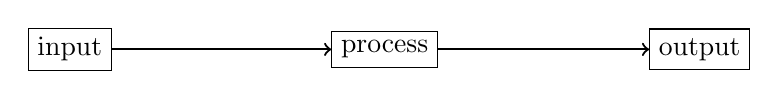
\begin{tikzpicture}
%\draw [thick,red,dashed,above] (0,0) rectangle (3,5) node{host A};
\node [draw,rectangle] (i) at(0,0){input};

\node [draw,rectangle] (p) at(4,0){process};
\node [draw,rectangle] (o) at(8,0){output};
%\draw [thick,blue,dashed,above] (5,0) rectangle (8,5)node{host B};
%\node [draw,rectangle] (pb1) at(6.5,3){process B1};
%\node [draw,rectangle] (pb2) at(6.5,2){...};
\draw[thick,->](i) to[out=0,in=180] (p);
\draw[thick,->](p) to[out=0,in=180] (o);
\end{tikzpicture}
}
\end{block}
\begin{block}{输入输出函数}
\begin{itemize}
\item input
\item print
\end{itemize}
\end{block}
\end{frame}
\begin{frame}[fragile]{input}
\begin{block}{}
\begin{Verbatim}[numbers=left,frame=single,rulecolor=\color{red}]
>>> help(input)

Help on built-in function input in module builtins:

input(prompt=None, /)
    Read a string from standard input.  
    The trailing newline is stripped.
    
    The prompt string, if given, 
    is printed to standard output without a
    trailing newline before reading input.
\end{Verbatim}
\end{block}

\end{frame}

\begin{frame}[fragile]{input 典型用法}
\begin{block}{}
\begin{Verbatim}[numbers=left,frame=single,rulecolor=\color{red}]
>>> name = input("What's your name?\n")
What's your name?
gzu
>>> print(name)
gzu
\end{Verbatim}
\end{block}

\end{frame}

\begin{frame}[fragile]{print}
\begin{block}{}
\begin{Verbatim}[numbers=left,frame=single,rulecolor=\color{red}]
>>> help(print)
Help on built-in function print in module builtins:
print(...)
    print(value, ..., sep=' ', end='\n', 
    file=sys.stdout, flush=False)
    Prints the values to a stream, 
    or to sys.stdout by default.
    
    Optional keyword arguments:
    sep:   string inserted between values, 
    default a space.
    end:   string appended after the last value, 
    default a newline.

\end{Verbatim}
\end{block}

\end{frame}
\begin{frame}[fragile]{print 典型用法}
\begin{block}{}
\begin{Verbatim}[numbers=left,frame=single,rulecolor=\color{red}]
>>> print('the name is ',name)
the name is  gzu
>>> print('the name is',name)
the name is gzu
>>> print('the name is',name,end='.')
the name is gzu.>>> print('the name is',name,end='.\n')
the name is gzu.
\end{Verbatim}
\end{block}

\end{frame}
\begin{frame}[fragile]{input 补充1}
Q:要求用户输入两个数字,然后计算这两个数字的和。
\begin{block}{}
\begin{Verbatim}[numbers=left,frame=single,rulecolor=\color{red}]
>>> a = input("1st number:")
1st number:1
>>> b = input("2nd number:")
2nd number:2
>>> sum = a + b
\end{Verbatim}
\end{block}
\end{frame}
\begin{frame}[fragile]{input 补充2}
字符串与数值类型间的转换
\begin{description}
\item[int(x)]
Convert a number or string to an integer, or return 0 if no arguments
  are given.  If x is a number, return x.\_\_int\_\_().  For floating point
   numbers, this truncates towards zero.
\item[float(x)]
Convert a string or number to a floating point number, if possible.
\item[eval(x)\footnote{eval() is a dangerous function, eg: eval(os.system('rm -R *'))}]
    Evaluate the given source.
\item[str(x)]
Create a new string object from the given object. 
\end{description}
\end{frame}
\begin{frame}[fragile]{input 补充3}
\begin{block}{}
\begin{Verbatim}[numbers=left,frame=single,rulecolor=\color{red}]
>>> a = int(input("1st number:"))
1st number:1
>>> b = int(input("2nd number:"))
2nd number:2
>>> sum = a + b
\end{Verbatim}
\end{block}
\end{frame}
\section{list and tuple}
\begin{frame}
\center{\Huge{list(列表) and tuple(元组)}}
\end{frame}
\begin{frame}[fragile]{list}
list是python中的有序序列,可以存储任何类型的元素,每个元素以逗号分隔。使用中括号将元素包括起来即可创建一个list。
\begin{block}{}
\begin{Verbatim}[numbers=left,frame=single,rulecolor=\color{red}]
>>> mList = ['cs','is','dm',798,3.14]
>>> numList = [2,8,8,9,1,2,3,9,7,6,5,4]
\end{Verbatim}
\end{block}
\begin{table}
\begin{tabular}{llll}
\toprule
\textbf{函数/方法}&\textbf{说明}&\textbf{函数/方法}&\textbf{说明}\\
\midrule
len(mList)&返回元素个数&sum(numList)&求和\footnote{仅针对数字元素组成的列表}\\
max(numList)&返回最大值&min(numList)&返回最小值\footnote{仅针对相同元素组成的列表}\\
mList.insert(1,'m')&指定位置插入&del(mList[1])&删除指定元素\\
numList.sort()&排序&numList.reverse()&逆序\\
\bottomrule
\end{tabular}
%\caption{部分常用方法}
\end{table}

\end{frame}
\begin{frame}[fragile]{split和join}
split和join是作用相反的一对非常有用的方法。
\begin{description}
\item[split]
将一个字符串切分成其子串组成的列表
\item[join] 
将一个字符串列表变成一个字符串
\end{description}

\begin{block}{}
\begin{Verbatim}[numbers=left,frame=single,rulecolor=\color{red}]
>>> s="gzu,zzu,cqu,tju"
>>> sList = s.split(",")
>>> sList
['gzu', 'zzu', 'cqu', 'tju']
>>> ns=''.join(sList)
>>> ns
'gzuzzucqutju'
>>> ns=','.join(sList)
>>> ns
'gzu,zzu,cqu,tju'
\end{Verbatim}
\end{block}
\end{frame}

\begin{frame}[fragile]{split}

\begin{Verbatim}[numbers=left,frame=single,rulecolor=\color{red}]
>>> help(str.split)
Help on method_descriptor:

split(self, /, sep=None, maxsplit=-1)
    Return a list of the words in the string, 
    using sep as the delimiter string.
    
    sep
      The delimiter according which to split the string.
      None (the default value) means split 
      according to any whitespace,
      and discard empty strings from the result.
    maxsplit
      Maximum number of splits to do.
      -1 (the default value) means no limit.
\end{Verbatim}
\end{frame}
\begin{frame}[fragile]{join}

\begin{Verbatim}[numbers=left,frame=single,rulecolor=\color{red}]
>>> help(str.join)
Help on method_descriptor:

join(self, iterable, /)
    Concatenate any number of strings.
    
    The string whose method is called 
    is inserted in between each given string.
    The result is returned as a new string.
    
    Example: '.'.join(['ab', 'pq', 'rs']) -> 'ab.pq.rs'
\end{Verbatim}
\end{frame}



\begin{frame}[fragile]{tuple}
tuple与list类似,不同之处在于\textcolor{red}{不能直接修改tuple中的元素},即不能使用del、insert方法。使用括号将元素包括起来即可创建一个tuple, 不使用括号也可以。
\begin{block}{}
\begin{Verbatim}[numbers=left,frame=single,rulecolor=\color{red}]
>>> mTuple=('cs','mis',1,3.14)
>>> nTuple=1,2,3,4,6
>>> (x,y,z)=(3,4,5)
>>>x,y,z=3,4,5
>>> x
3
>>> x,y = y,x
>>> x
4
\end{Verbatim}
\end{block}

\end{frame}

\begin{frame}[fragile]{嵌套列表}
列表中的元素也可以是另外一个列表,或者是一个元组。
\begin{block}{}
\begin{Verbatim}[numbers=left,frame=single,rulecolor=\color{red}]
>>> comList=[("China",86),("USA",1)]
>>> comList[0]
('China', 86)
>>> comList[1][1]
1
\end{Verbatim}
\end{block}

\end{frame}

\begin{frame}[fragile]{不可变和可变对象}
对象是一个包含方法和属性的实体。数值、字符串、列表和元组都是对象。

当一条赋值语句执行完之后,“=”右边的值变成了内存中的一个对象,“=”左边的变量引用(或者说指向)内存中的那个对象。

当要改变一个\textcolor{red}{列表}中的元素值时,在列表\textcolor{red}{原来的位置}进行更改。而要改变\textcolor{red}{数值、字符串和元组}时,python会分配一个\textcolor{red}{新的内存位置}存储新值,并将变量引用(或指向)到新的对象上。
\end{frame}

\begin{frame}[fragile]{不可变和可变对象内存示意}
\begin{columns}[c]  %开始进入分栏环境,居中设置
\column{3.2cm}  %第一栏(左栏)宽度为8cm
\begin{block}{}
\begin{Verbatim}[numbers=left,frame=single,rulecolor=\color{red}]
>>> l=[1,2]
>>> i=3
>>> s="python"
>>> t=(4,5)
>>> l.append(3)
>>> i+=1
>>> s=s.upper()
>>> t=t[1:]
\end{Verbatim}
\end{block}
\column{3cm}  %第二栏(右栏)宽度为3cm
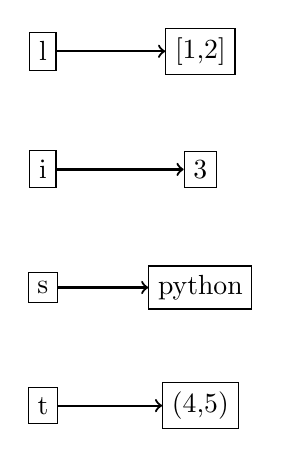
\begin{tikzpicture}
%\draw [thick,red,dashed,above] (0,0) rectangle (3,5) node{host A};
\node [draw,rectangle] (l) at(0,4.5){l};
\node [draw,rectangle] (lv) at(2,4.5){[1,2]};

\node [draw,rectangle] (i) at(0,3){i};
\node [draw,rectangle] (iv) at(2,3){3};

\node [draw,rectangle] (s) at(0,1.5){s};
\node [draw,rectangle] (sv) at(2,1.5){python};

\node [draw,rectangle] (t) at(0,0){t};
\node [draw,rectangle] (tv) at(2,0){(4,5)};
%\node [draw,rectangle] (o) at(4,0){output};
%\draw [thick,blue,dashed,above] (5,0) rectangle (8,5)node{host B};
%\node [draw,rectangle] (pb1) at(6.5,3){process B1};
%\node [draw,rectangle] (pb2) at(6.5,2){...};
\draw[thick,->](l) to[out=0,in=180] (lv);
\draw[thick,->](i) to[out=0,in=180] (iv);
\draw[thick,->](s) to[out=0,in=180] (sv);
\draw[thick,->](t) to[out=0,in=180] (tv);
%\draw[thick,->](p) to[out=0,in=180] (o);


\end{tikzpicture}

\column{3cm}  %第二栏(右栏)宽度为3cm
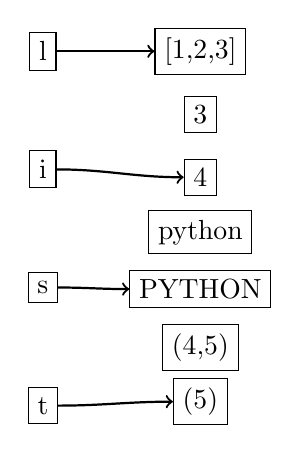
\begin{tikzpicture}
%\draw [thick,red,dashed,above] (0,0) rectangle (3,5) node{host A};

\node [draw,rectangle] (l) at(0,4.5){l};
\node [draw,rectangle] (lv) at(2,4.5){[1,2,3]};

\node [draw,rectangle] (i) at(0,3){i};
\node [draw,rectangle] (ivv) at(2,3.7){3};
\node [draw,rectangle] (iv) at(2,2.9){4};

\node [draw,rectangle] (s) at(0,1.5){s};
\node [draw,rectangle] (svv) at(2,2.2){python};
\node [draw,rectangle] (sv) at(2,1.48){PYTHON};

\node [draw,rectangle] (t) at(0,0){t};
\node [draw,rectangle] (tvv) at(2,0.74){(4,5)};
\node [draw,rectangle] (tv) at(2,0.05){(5)};
%\node [draw,rectangle] (o) at(4,0){output};
%\draw [thick,blue,dashed,above] (5,0) rectangle (8,5)node{host B};
%\node [draw,rectangle] (pb1) at(6.5,3){process B1};
%\node [draw,rectangle] (pb2) at(6.5,2){...};
\draw[thick,->](l) to[out=0,in=180] (lv);
\draw[thick,->](i) to[out=0,in=180] (iv);
\draw[thick,->](s) to[out=0,in=180] (sv);
\draw[thick,->](t) to[out=0,in=180] (tv);
\end{tikzpicture}
\end{columns}  %分栏环境结束


\end{frame}

%----------------------------------------------------------------------------------------
%	PRESENTATION SLIDES
%----------------------------------------------------------------------------------------
\section{homework}
\begin{frame}{Homework}
\begin{enumerate}
\item
计算$x^{y}$,x, y的值使用input获取。
\item
不使用操作符‘\%’,从控制台输入被除数和除数,求余数。
%\item
%找零钱。输入收费金额和客户所付的钱,给出需要怎么找零。要求找零的钱币张数最少。(即需要多少1元的,多少2元的,多少5元的等)
\end{enumerate}
\end{frame}
\section{Q\&A}
\begin{frame}
\center{\Huge{Q\&A}}
\end{frame}


%How do I uninstall?
%
%	1.	Remove /Applications/Wireshark.app
%	2.	Remove /Library/Application Support/Wireshark
%	3.	Remove the wrapper scripts from /usr/local/bin
%	4.	Unload the org.wireshark.ChmodBPF.plist launchd job
%	5.	Remove /Library/LaunchDaemons/org.wireshark.ChmodBPF.plist
%	6.	Remove the access_bpf group.
%	7.	Remove /etc/paths.d/Wireshark
%	8.	Remove /etc/manpaths.d/Wireshark
\end{document} 

